\subsection{Background}
Wavelets are mathematical tools that are often used in the context of signal processing. They were introduced by Alfréd Haar in 1909\cite{haar} and wavelet theory was later expanded by multiple mathematicians, including Stéphane Mallat and Ingrid Daubechies. Wavelet transforms can be viewed as a generalization of Fourier transforms. While the latter only contain frequency information, the former capture information about location in time as well. Both continous and discrete wavelet transforms (DWT) admit an inverse transform.

DWTs and inverse discrete wavelet transforms (IDWT) are often used in the contexts of computer vision\cite{wavelet_application_4} and image processing\cite{wavelet_application_1}\cite{wavelet_application_2}, both for image compression and denoising\cite{wavelet_application_3}. In particular, the 5/3 and 9/7 wavelet transforms are used in the JPEG 2000 standard, for reversible and irreversible compression respectively, achieving both a higher compression rate and higher image quality over JPEG.

In the simplest implementation of a DWT, a signal is convolved with a low-pass and a high-pass filter. A more efficient implementation which uses a lifting scheme was proposed by Wim Sweldens\cite{lifting}. While 1D DWTs have a computational complexity of $O(n)$, 2D DWTs require computing the DWT of each row and each column of the input and are often the main computational kernel in applications that use them. As such, multiple works that focus on optimizing DWT computations have been proposed\cite{wavelet_fast_1}\cite{wavelet_fast_2}\cite{wavelet_fast_3}\cite{wavelet_fast_4}.

A 1-level 2D DWT consist in applying a 1D DWT to all rows in the input matrix and then to all columns of the partial result. The resulting coefficients can be divided into four sets, based on which pixels contain low or high-passed data. These sets are denoted as LL, HL, LH and HH and can be visualized as an image like in Figure \ref{fig:castle_level1}, where the top-left quadrant contains the data in the LL set. A multi-level 2D DWT consists in iteratively applying a 1-level DWT to the LL quadrant of the previous result.

\subsection{Code structure and functionalities}
Most wavelet-related functionalities are declared in \texttt{Wavelet\-Transform.hpp} and implemented in \texttt{Wavelet\-Transform.cpp}. An abstract class \texttt{Wavelet\-Transform\-Algorithm} representing a 1D wavelet transform algorithm with two virtual methods \texttt{direct\-Transform} and \texttt{inverse\-Transform} is declared. Two concrete classes inherit from it, overriding its methods. Moreover, a \texttt{Two\-Dimensional\-Wavelet\-Transform\-Algorithm} class is declared. Said class is passed a unique pointer to a \texttt{Wavelet\-Transform\-Algorithm} as a constructor argument and specifies two public methods for performing a multi-level 2D DWT and IDWT using the provided 1D algorithm.

\texttt{Grayscale\-Image.cpp} contains the definitions of two more wavelet-related methods: \texttt{wavelet\-Transform} and \texttt{denoise}, used to apply a 2D DWT to the image and visualize the result and to denoise an image respectively.

Finally, wavelet-related functionalities are used in \texttt{wavelet\_main.cpp}.

The two concrete 1D wavelet transform classes provide two implementations of the 9/7 DWT and IDWT. The first version \texttt{GP\-Wavelet\-Transform\-97} was adapted from C code by Gregoire Pau\cite{gregoire_pau} and rewritten in modern C++. The second implementation \texttt{Daubechies\-Wavelet\-Transform\-97} was developed following the descriptions in \cite{daubechies} and \cite{wavelet_fast_1}. Since the reported articles do not specify how to treat the first and last value in the high and low passed sequences, the same approach as the previously mentioned implementation was used. The two DWT implementations do not provide identical transforms for the same sequences. Due to the lack of complete and reliable documentation, we were unable to establish which implementation corresponds to the real 9/7 DWT, as both implementations provide valid results in their applications to image processing.

Wavelet code was written with the objectives of readability and expandability, but no in-depth performance analysis was performed. Additionally, the 2D algorithms use conditional OpenMP parallelization over the rows and columns of the input. While the DWT and IDWT implementations of \texttt{Daubechies\-Wavelet\-Transform\-97} are parallelizable as well, parallelization was avoided, as consumer-grade architectures have a number of processors that is far lower than the amount that would benefit from this nested parallelization.

\subsection{Results}
As a proof of concept, we applied the 2D algorithms to some images, obtaining the following results.

The first test case is aimed at reproducing \cite{castle}, where the image was further processed for displaying purposes, achieving more visible details in the darker quadrants. An instance of \texttt{Daubechies\-Wavelet\-Transform\-97} was applied to the image in Figure \ref{fig:castle_original}. The resulting coefficients where then mapped into the range [0, 255] using an affine map and interpreted as pixel values, obtaining the results in Figure \ref{fig:castle_level1} and \ref{fig:castle_level2}. The LL quadrant contains an image similar to the original one. Despite the fact that other quadrants are dark, when zooming it, the sharp edges in the original image can be seen. This example shows one of the advantages of DWTs over DFTs, i.e. the ability to extract information about sharp changes in an image, which the human eye is very susceptible to.

\begin{figure}[h]
    \centering
    \subfigure[Original]{\label{fig:castle_original}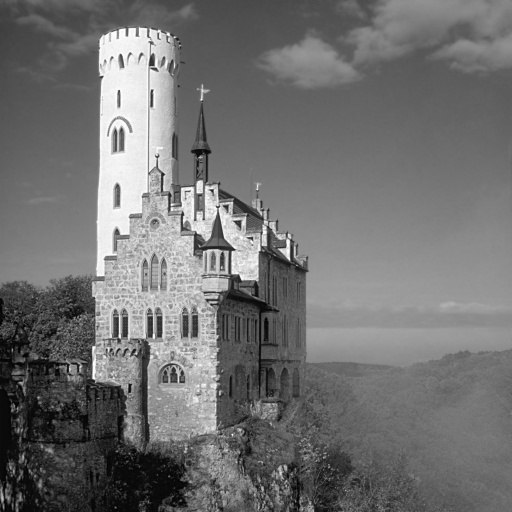
\includegraphics[width=35mm]{image/castle_original}}
    \subfigure[1-level DWT]{\label{fig:castle_level1}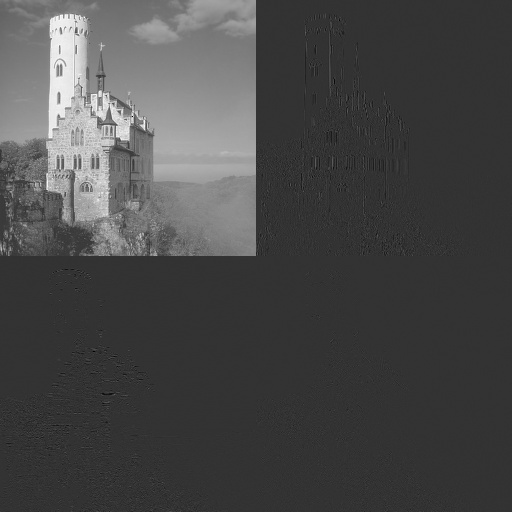
\includegraphics[width=35mm]{image/castle_level1}}
    \subfigure[2-level DWT]{\label{fig:castle_level2}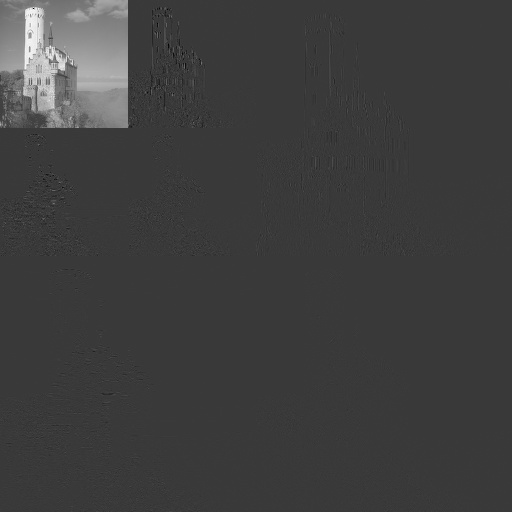
\includegraphics[width=35mm]{image/castle_level2}}
    \caption{Multi level DWT applied to an example image.}
    \label{fig:wavelet_2d}
\end{figure}

The second test case shows the possible application of wavelet transforms to denoising. We applied a multi-level DWT to an image, performed a thresholding step, and then performed the IDWT. Hard thresholding consists in setting to 0 all values below the given threshold, while soft thresholding does the same and additionally reduces the absolute value of the remaining values by the threshold. While advanced denoising algorithms use more complicated steps, for simple applications like the image in Figure \ref{fig:noise_original}, our algorithm can remove most of the Gaussian noise in the original image, as shown in Figure \ref{fig:thresholding}. Figure \ref{fig:noise_hard} was obtained with a 1-level DWT with hard thresholding with threshold 80, while Figure \ref{fig:noise_soft} was obtained with a 4-level DWT and soft thresholding with threshold 30. Both results use an instance of \texttt{GP\-Wavelet\-Transform\-97}. 

\begin{figure}[h]
    \centering
    \subfigure[Original]{\label{fig:noise_original}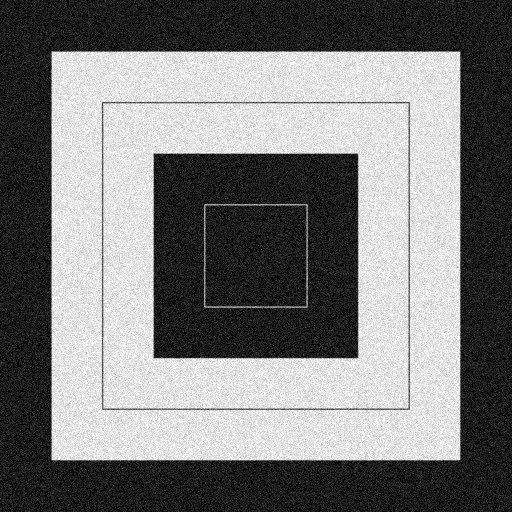
\includegraphics[width=35mm]{image/noise_original}}
    \subfigure[Hard thresholding]{\label{fig:noise_hard}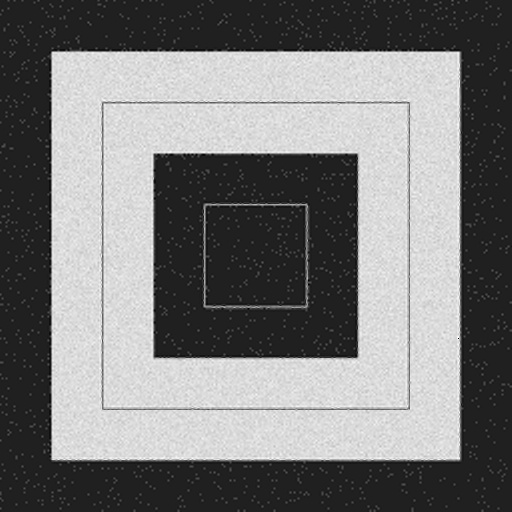
\includegraphics[width=35mm]{image/noise_hard}}
    \subfigure[Soft thresholding]{\label{fig:noise_soft}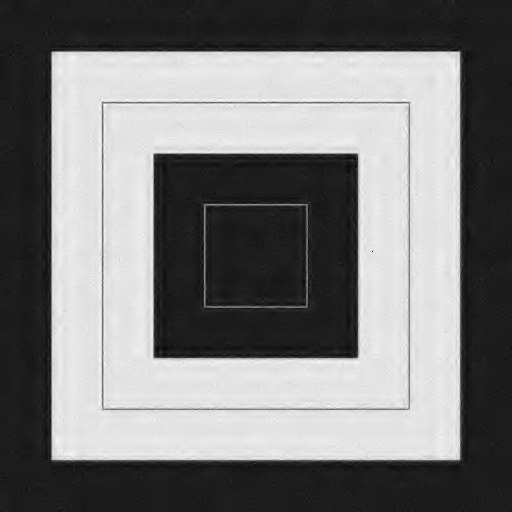
\includegraphics[width=35mm]{image/noise_soft}}
    \caption{DWT and thresholding applied to an example image.}
    \label{fig:thresholding}
\end{figure}